\documentclass[12pt,a4paper]{article}

% Encoding & language
\usepackage[utf8]{inputenc}
\usepackage[T1]{fontenc}
\usepackage[main=english]{babel}
\usepackage{caption}
\usepackage{booktabs}

% untuk kode
\usepackage{listings}

% Margin & spacing
\usepackage{geometry}
\geometry{margin=1in}
\usepackage{setspace}
\setstretch{1.2}

% Math & extras
\usepackage{enumitem}
\usepackage{amsmath,amssymb,amsthm}
\usepackage{algorithm}
\usepackage{algpseudocode}

\theoremstyle{remark}
\newtheorem*{solusi}{Solusi}

% Paket untuk gambar
\usepackage{graphicx}
\usepackage{tikz}
\usetikzlibrary{shapes.geometric, arrows, positioning}
\usetikzlibrary{calc}

% Etc
\usepackage{titling}
\usepackage{csquotes}
\usepackage{subcaption}
% Untuk hyperlink
\usepackage{hyperref}

% --- Biblatex dengan IEEE style ---
\usepackage[backend=biber,style=ieee,language=english]{biblatex}
\addbibresource{refs.bib}

\DefineBibliographyStrings{english}{%
  references   = {Daftar Pustaka},
  bibliography = {Daftar Pustaka},
  and          = {dan},
  andothers    = {dkk.},
  pages        = {hlm.},
}

% STYLING
\setlength{\parindent}{2em}

% OVERRIDE Caption
\captionsetup[figure]{labelfont=bf, name=Gambar, justification=centering}
\captionsetup[table]{labelfont=bf, name=Tabel, justification=centering}



% --- Title page ---
\title{%
  \textbf{Tugas Mata Kuliah} \\
  \large Rekayasa Fitur dan Pengenalan Pola (RFPP) \\
  \large Klasifikasi Melanoma dengan Pendekatan \textit{Hand-crafted Features} \\ dan Pemelajaran Mesin}
  
\author{Khalilullah Al Faath \\ NIU: 566643 \\ Magister Ilmu Komputer \\ [1cm]
  \includegraphics[width=0.4\textwidth]{images/logo-ugm.png}}
\date{Universitas Gadjah Mada \\ Semester Gasal 2025/2026}

\makeatletter
\renewcommand{\maketitle}{%
  \begin{titlepage}
    \centering
    \vspace*{2cm}
    
    {\LARGE \@title \par}
    \vspace{2cm}
    
    {\large \@author \par}
    
    \vfill
    
    {\large \@date \par}
  \end{titlepage}
}
\makeatother

\begin{document}

\maketitle
\thispagestyle{empty}

% Daftar isi dan daftar gambar/tabel

% override label
\renewcommand{\contentsname}{Daftar Isi}
\renewcommand{\listfigurename}{Daftar Gambar}
\renewcommand{\listtablename}{Daftar Tabel}

% daftar isi
\tableofcontents

\newpage

% daftar gambar
\listoffigures

\newpage

% daftar tabel
\listoftables

\newpage
\setcounter{page}{1}

\section{Pendahuluan}
Melanoma maligna merupakan bentuk neoplasma kulit yang paling mematikan yang merupakan hasil transformasi melanosit, yaitu sel yang berasal dari \textit{neural crest}. Karena asal-usul embriologisnya, melanoma tidak hanya terbatas pada kulit, tetapi juga dapat berkembang di lokasi lain tempat sel \textit{neural crest} bermigrasi, seperti traktus gastrointestinal, otak, dan mata (melanoma okular). Secara patofisiologis, perkembangan melanoma sangat dipengaruhi oleh faktor lingkungan (terutama paparan radiasi UV), genetik (seperti mutasi pada gen BRAF, CDKN2A, CDK4), dan imunologis \cite{heistein_malignant_2025}.

Urgensi pengembangan sistem deteksi dan klasifikasi melanoma didasari oleh tren peningkatan insiden dan risiko fatalitas yang yang tinggi. Berdasarkan data \textit{National Cancer Instite (NCI) Surveillance, Epidemiology, and End Results (SEER)}, (1) melanoma kini  merupakan kanker ganas yang paling umum yang terjadi di pria dan wanita, (2) pada tahun 2023, diperkirakan terdapat 97.000 kasus baru di Amerika Serikat dengan estimasi 7.990 kematian \cite{siegel_cancer_2023}, (3) Tingkat kelangsungan hidup relatif 5 tahun (5-year relative survival rate) sangat bergantung pada stadium saat diagnosis: pasien dengan melanoma stadium 0 (in-situ) memiliki tingkat kelangsungan hidup mencapai 97\% hingga 100\%. Sebaliknya, angka ini menurun drastis menjadi sekitar 30\% hingga 52\% bagi pasien yang terdiagnosis pada stadium IV (metastatik) \cite{heistein_malignant_2025}, (4) di Indonesia, pada tahun 2020, angka kasus kanker kulit mencapai 18.000 kasus dengan angka kematian sekitar 3.000 \cite{primaya_hospital_editor_kanker_2023}.

Deteksi dini melanoma dapat dilakukan dengan menggunakan metode jembatan keledai "ABCDE", yaitu "A" untuk \textit{Asymmetry} atau asimetris, "B" untuk \textit{Border} atau tepi, "C" untuk \textit{color} atau warna, "D" untuk \textit{Diameter}, dan "E" untuk \textit{Evolving} atau berevolusi \cite{heistein_malignant_2025}. Gambar~\ref{fig:abcde} menggambarkan karakteristik khusus dari melanoma.

\begin{figure}[H]
  \centering
  \includegraphics[width=0.75\linewidth]{images/abcde-melanoma.png}
  \caption{Karakteristik Melanoma}
  \label{fig:abcde}
\end{figure}

Pengembangan sistem \textit{Computer-Aided Diagnosis (CAD)} untuk deteksi melanoma telah menjadi fokus penelitian intensif dalam beberapa dekade terakhir. Secara garis besar, penelitian-penelitian sebelumnya dapat dikelompokkan menjadi dua pendekatan utama: metode berbasis ekstraksi fitur manual atau (\textit{hand-crafted features}) dan metode berbasis pemelajaran dalam atau \textit{Deep Learning}.

\begin{description}
  \item[Pendekatan ekstraksi manual] Pendekatan pertama, yaitu metode ekstraksi fitur manual, berfokus pada pemodelan karakteristik visual melanoma berdasarkan pengetahuan klinis dan aturan morfologi. Pada pendekatan ini, proses analisis citra dilakukan melalui tahapan pra-pemrosesan, segmentasi lesi, dan ekstraksi fitur berbasis ciri geometris, tekstur, atau warna. Contohnya termasuk penggunaan fitur statistik orde pertama, \textit{Histogram of Oriented Gradients (HOG)}, \textit{Local Binary Patterns (LBP)}, momen bentuk, hingga parameter geometrik seperti asimetri, \textit{compactness}, dan \textit{eccentricity}. Pendekatan ini memiliki keunggulan berupa interpretabilitas yang tinggi karena parameter yang dianalisis selaras dengan kriteria klinis seperti aturan ABCDE. Namun, performanya sangat bergantung pada kualitas segmentasi dan sensitivitas model terhadap variasi perangkat fotografi, pencahayaan, serta keberadaan artefak seperti rambut, bayangan, dan variasi kulit \cite{tumpa_artificial_2021, mahum_skin_2022, almaraz-damian_melanoma_2020}.
  \item[Pendekatan pemelajaran dalam] Sebaliknya, pendekatan berbasis pemelajaran dalam (\textit{Deep Learning}) memanfaatkan jaringan saraf tiruan berlapis banyak, khususnya \textit{Convolutional Neural Network} (CNN), untuk mengekstraksi representasi fitur secara otomatis tanpa memerlukan desain fitur manual oleh pakar. Model seperti ResNet, EfficientNet, dan Vision Transformer (ViT) telah menunjukkan performa unggul dalam kompetisi internasional seperti International Skin Imaging Collaboration (ISIC). Keunggulan utama pendekatan ini adalah kemampuannya untuk belajar dari data berskala besar, mengurangi ketergantungan pada pra-pemrosesan, serta meningkatkan robustnes terhadap variasi pola, warna, dan tekstur lesi kulit. Namun, tantangannya mencakup kebutuhan dataset besar yang teranotasi dengan baik, risiko bias algoritmik akibat ketidakseimbangan distribusi data (misalnya warna kulit pasien), serta keterbatasan interpretabilitas (\textit{black-box problem}) \cite{esteva_dermatologist-level_2017,li_skin_2017, wu_skin_2022}.
\end{description}

Klasifikasi melanoma yang dilakukan pada tugas ini dilakukan dengan menggunakan ekstraksi fitur manual dengan model pemelajaran mesin \textit{Support Vector Machine} (SVM).

\section{Metode}
Bagian ini menjelaskan alur langkah yang dilakukan pada tugas ini. Gambar~\ref{fig:diagramalir} menunjukkan alur langkah metode yang diusulkan.

\begin{figure}[H]
  \centering
  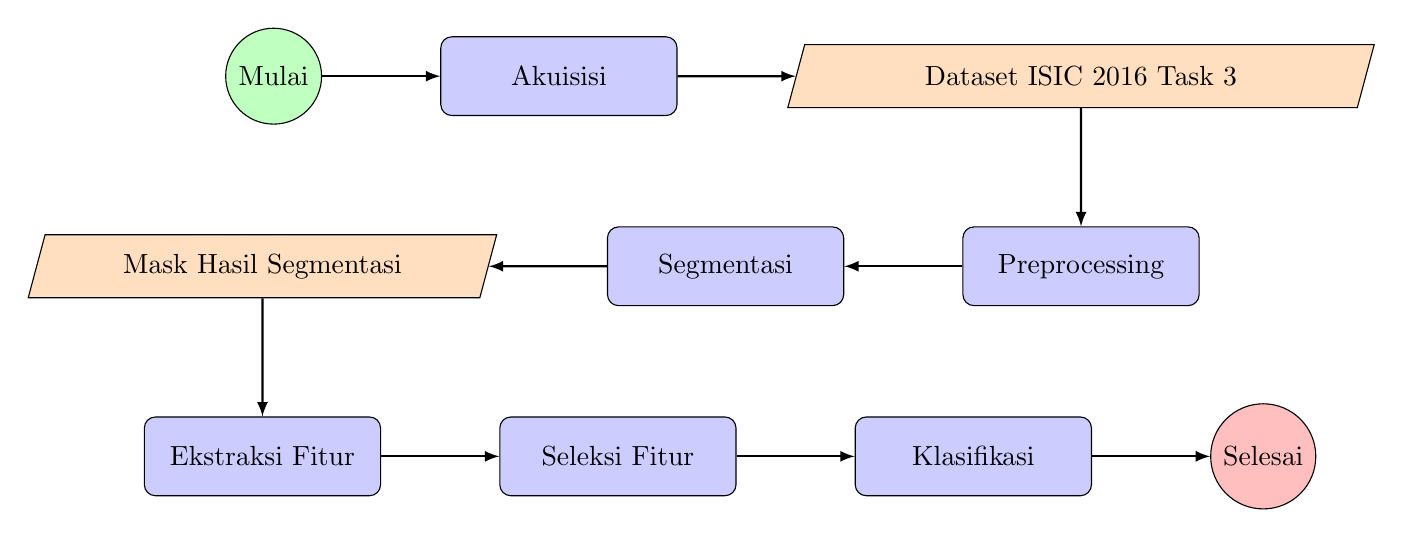
\begin{tikzpicture}[
      node distance=15mm,
      proc/.style={
          rectangle,
          draw,
          rounded corners,
          align=center,
          minimum width=30mm,
          minimum height=10mm,
          fill=blue!20
        },
      io/.style={
          trapezium,
          trapezium left angle=75,
          trapezium right angle=105,
          draw,
          align=center,
          minimum width=25mm,
          minimum height=8mm,
          fill=orange!25
        },
      term-start/.style={
          circle,
          draw,
          align=center,
          minimum size=10mm,
          fill=green!25
        },
      term-finish/.style={
          circle,
          draw,
          align=center,
          minimum size=10mm,
          fill=red!25
        },
      arrow/.style={
          -latex,
          thick
        }
    ]

    % Nodes
    \node[term-start] (mulai) {Mulai};
    \node[proc, right=of mulai] (akuisisi) {Akuisisi};
    \node[io, right=of akuisisi] (isic) {Dataset ISIC 2016 Task 3};
    \node[proc, below=of isic] (pre) {Preprocessing};
    \node[proc, left=of pre] (seg) {Segmentasi};
    \node[io, left=of seg] (mask) {Mask Hasil Segmentasi};
    \node[proc, below=of mask] (ekstrak) {Ekstraksi Fitur};
    \node[proc, right=of ekstrak] (seleksi) {Seleksi Fitur};
    \node[proc, right=of seleksi] (klasif) {Klasifikasi};
    \node[term-finish, right=of klasif] (selesai) {Selesai};

    % Arrows
    \draw[arrow] (mulai) -- (akuisisi);
    \draw[arrow] (akuisisi) -- (isic);
    \draw[arrow] (isic) -- (pre);
    \draw[arrow] (pre) -- (seg);
    \draw[arrow] (seg) -- (mask);
    \draw[arrow] (mask) -- (ekstrak);
    \draw[arrow] (ekstrak) -- (seleksi);
    \draw[arrow] (seleksi) -- (klasif);
    \draw[arrow] (klasif) -- (selesai);

  \end{tikzpicture}
  \caption{Diagram alir metode yang dilakukan}
  \label{fig:diagramalir}
\end{figure}





\subsection{Akuisisi}\label{section:dataset}
Dataset yang digunakan pada tugas ini adalah Dataset ISIC 2016 Task 3. \footnote{Dataset ini dapat diunduh di pranala berikut \url{https://challenge.isic-archive.com/landing/2016/39/}} Dataset ini merupakan himpunan citra dermoskopik yang digunakan untuk menyelesaikan permasalahan klasifikasi lesi kulit menjadi dua kategori, yaitu \textit{benign} (non-malignant) dan \textit{malignant}. Gambar~\ref{fig:contoh-data} menunjukkan contoh data yang ada pada Dataset, sementara Gambar~\ref{fig:contoh-benign} menunjukkan contoh citra berlabel \textit{benign} dan \textit{malignant}.

\begin{figure}[H]
  \centering
  \includegraphics[trim=0 5cm 0 3cm, clip, width=1\textwidth]{images/contoh-data.pdf}
  \caption{Contoh citra yang ada pada Dataset ISIC 2016 Task 3.}
  \label{fig:contoh-data}
\end{figure}

\begin{figure}[H]
  \centering
  \includegraphics[trim=0 5cm 0 3cm, clip, width=1\textwidth]{images/contoh-benign.pdf}
  \caption{Contoh citra \textit{benign} dan \textit{malignant}.}
  \label{fig:contoh-benign}
\end{figure}

Dataset pelatihan terdiri atas 900 citra lesi kulit dalam format JPEG dengan resolusi bervariasi. Setiap citra dinamai menggunakan pola \texttt{ISIC\_<image\_id>.jpg} dengan tujuh digit pengenal unik. Berkas pelatihan dilengkapi dengan \textit{Training Ground Truth} berupa sebuah berkas CSV yang memuat dua kolom: (1) \texttt{image\_id} yang sesuai dengan nama berkas citra, dan (2) label diagnosis definitif (\textit{benign} atau \textit{malignant}) yang ditentukan berdasarkan konsensus pakar serta laporan patologi.

Selain itu, disediakan pula seperangkat \textit{Test Data} yang terdiri dari 379 citra dengan format yang sama. Berbeda dengan data pelatihan, data uji tidak disertai label kebenaran untuk menjaga objektivitas evaluasi. Pada proses kompetisi aslinya, peserta diminta mengunggah hasil prediksi dalam format CSV dua kolom berisi \texttt{image\_id} dan skor probabilistik dalam rentang [0.0, 1.0], dengan nilai di atas 0.5 mengindikasikan prediksi \textit{malignant} \cite{isic_committee_isic_2016}.

Dapat dilihat pada Gambar~\ref{fig:contoh-data} terdapat beberapa jenis \textit{noice} yang dapat diidentifikasi, yaitu \textit{border noice}, \textit{hair noice}, dan \textit{object noice}.

\subsection{\textit{Pre-processing}}
Setelah mendapatkan Dataset, dilakukan \textit{pre-processing} atau pra-pemrosesan untuk menghilangkan sebagian noice. Gambar~\ref{fig:preprocessing} menunjukkan langkah-langkah pra-pemrosesan yang dilakukan.

\begin{figure}[H]
  \centering
  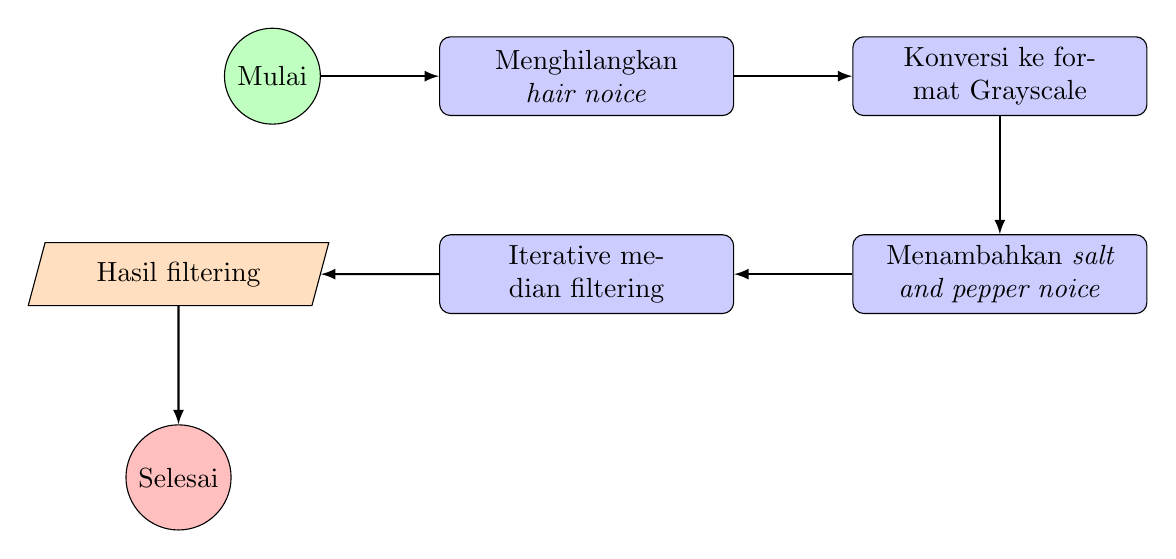
\begin{tikzpicture}[
      node distance=15mm,
      proc/.style={
          rectangle,
          draw,
          rounded corners,
          align=center,
          minimum width=30mm,
          minimum height=10mm,
          text width=35mm,
          fill=blue!20
        },
      io/.style={
          trapezium,
          trapezium left angle=75,
          trapezium right angle=105,
          draw,
          align=center,
          minimum width=25mm,
          minimum height=8mm,
          fill=orange!25
        },
      term-start/.style={
          circle,
          draw,
          align=center,
          minimum size=10mm,
          fill=green!25
        },
      term-finish/.style={
          circle,
          draw,
          align=center,
          minimum size=10mm,
          fill=red!25
        },
      arrow/.style={
          -latex,
          thick
        }
    ]

    % Nodes
    \node[term-start] (mulai) {Mulai};
    \node[proc, right=of mulai] (hair) {Menghilangkan \textit{hair noice}};
    \node[proc, right=of hair] (konversi) {Konversi ke format Grayscale};
    \node[proc, below=of konversi] (salt) {Menambahkan \textit{salt and pepper noice}};
    \node[proc, left=of salt] (filter) {Iterative median filtering};
    \node[io, left=of filter] (hasil) {Hasil filtering};
    \node[term-finish, below=of hasil] (selesai) {Selesai};

    % Arrows
    \draw[arrow] (mulai) -- (hair);
    \draw[arrow] (hair) -- (konversi);
    \draw[arrow] (konversi) -- (salt);
    \draw[arrow] (salt) -- (filter);
    \draw[arrow] (filter) -- (hasil);
    \draw[arrow] (hasil) -- (selesai);

  \end{tikzpicture}



  \caption{Diagram alir pra-pemrosesan.}
  \label{fig:preprocessing}
\end{figure}

Setiap tahap pra-pemrosesan memiliki tujuan spesifik untuk mempersiapkan citra sebelum dilakukan segmentasi dengan mengikuti alur dari penelitian \textcite{jaseema_yasmin_improved_2012}.

\begin{enumerate}
  \item \textbf{Menghilangkan \textit{hair noise}}: Pada citra dermoskopik, rambut yang menutupi lesi dapat mengganggu analisis dan segmentasi. Oleh karena itu, rambut dihilangkan menggunakan operasi morfologi \textit{black-hat} yang diikuti dengan \textit{inpainting} untuk menutupi area rambut dengan piksel sekitarnya, sehingga citra menjadi lebih bersih.

  \item \textbf{Konversi ke format Grayscale}: Citra RGB dikonversi menjadi citra intensitas (grayscale) untuk menyederhanakan data dan mengurangi kompleksitas komputasi. Dengan ini, analisis selanjutnya hanya fokus pada intensitas piksel, sehingga pengaruh variasi warna yang tidak relevan dapat diminimalkan.

  \item \textbf{Menambahkan \textit{salt and pepper noise}}: Tahap ini dilakukan untuk menyiapkan citra dalam kondisi yang memungkinkan pengujian ketahanan metode filter. Noise buatan ditambahkan pada citra grayscale agar metode \textit{iterative median filtering} dapat diuji efektivitasnya dalam menghilangkan noise dan mempertahankan tepi lesi.

  \item \textbf{Iterative Median Filtering}: Citra yang telah diberi noise kemudian difilter menggunakan metode median secara iteratif. Filter median efektif untuk menghilangkan noise impulsif (\textit{salt and pepper}) tanpa merusak kontur objek penting. Proses iteratif memastikan noise tersisa dapat dihilangkan secara bertahap, sambil mempertahankan detail lesi.

  \item \textbf{Hasil Filtering}: Tahap ini menghasilkan citra yang bersih dari noise, dengan kontur lesi tetap terjaga. Citra hasil ini siap digunakan untuk tahap segmentasi dan ekstraksi fitur selanjutnya.
\end{enumerate}

Gambar~\ref{fig:hasil-preprocessing} memperlihatkan contoh hasil tiap tahap filtering pada citra dermoskopik.

\begin{figure}[H]
  \centering
  \includegraphics[trim=0 5cm 0 3cm, clip, width=1\textwidth]{images/hasil-filtering.pdf}
  \caption{(1) Konversi ke Grayscale; (2) Menambahkan \textit{salt and pepper noice}; (3) Menerapkan \textit{Iterative median filtering}}
  \label{fig:hasil-preprocessing}
\end{figure}

\subsection{Segmentasi}
Setelah pra-pemrosesan, didapatkan citra hasil filtering yang siap untuk disegmentasi. Gambar~\ref{fig:segmentasi} menunjukkan tahapn segmentasi yang dilakukan.

\begin{figure}[H]
  \centering
  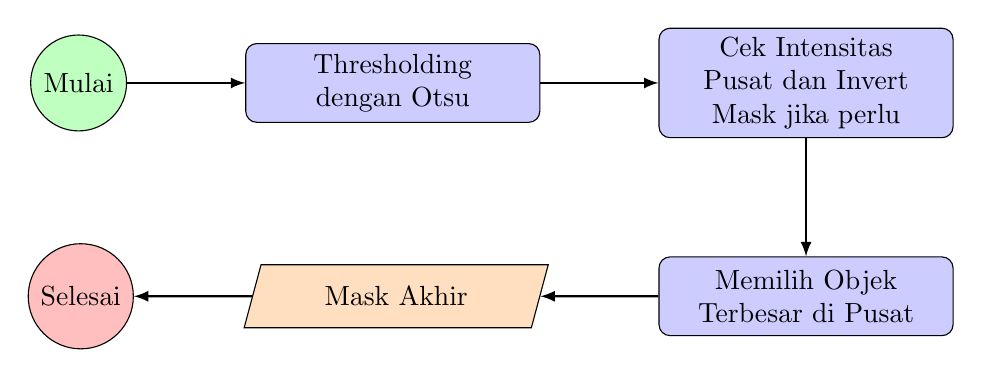
\begin{tikzpicture}[
      node distance=15mm,
      proc/.style={
          rectangle,
          draw,
          rounded corners,
          align=center,
          minimum width=30mm,
          minimum height=10mm,
          text width=35mm,
          fill=blue!20
        },
      io/.style={
          trapezium,
          trapezium left angle=75,
          trapezium right angle=105,
          draw,
          align=center,
          minimum width=25mm,
          minimum height=8mm,
          fill=orange!25
        },
      term-start/.style={
          circle,
          draw,
          align=center,
          minimum size=10mm,
          fill=green!25
        },
      term-finish/.style={
          circle,
          draw,
          align=center,
          minimum size=10mm,
          fill=red!25
        },
      arrow/.style={
          -latex,
          thick
        }
    ]

    % Nodes
    \node[term-start] (mulai) {Mulai};
    \node[proc, right=of mulai] (otsu) {Thresholding dengan Otsu};
    \node[proc, right=of otsu] (check) {Cek Intensitas Pusat dan Invert Mask jika perlu};
    \node[proc, below=of check] (keep) {Memilih Objek Terbesar di Pusat};
    \node[io, left=of keep] (save) {Mask Akhir};
    \node[term-finish, left=of save] (selesai) {Selesai};

    % Arrows
    \draw[arrow] (mulai) -- (otsu);
    \draw[arrow] (otsu) -- (check);
    \draw[arrow] (check) -- (keep);
    \draw[arrow] (keep) -- (save);
    \draw[arrow] (save) -- (selesai);

  \end{tikzpicture}



  \caption{Diagram alir segmentasi.}
  \label{fig:segmentasi}
\end{figure}

\subsubsection{\textit{Thresholding} dengan Otsu}
Citra hasil pra-pemrosesan difilter menggunakan metode threshold otomatis Otsu (\textit{Otsu's method}) untuk menghasilkan \textit{binary mask} awal (\textit{mask\_raw}). \textit{Threshold} Otsu secara adaptif menentukan nilai ambang yang memisahkan piksel gelap (lesi) dan terang (kulit) berdasarkan histogram intensitas, sehingga tidak perlu menentukan \textit{threshold} secara manual.

\begin{figure}[H]
  \centering
  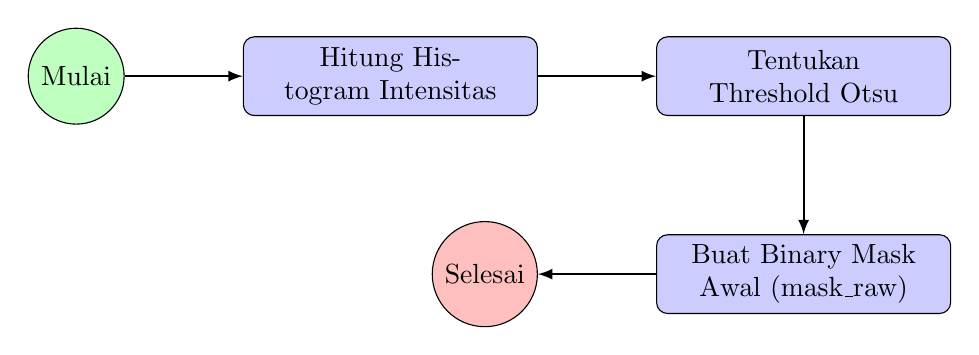
\begin{tikzpicture}[
      node distance=15mm,
      proc/.style={
          rectangle,
          draw,
          rounded corners,
          align=center,
          minimum width=30mm,
          minimum height=10mm,
          text width=35mm,
          fill=blue!20
        },
      io/.style={
          trapezium,
          trapezium left angle=75,
          trapezium right angle=105,
          draw,
          align=center,
          minimum width=25mm,
          minimum height=8mm,
          fill=orange!25
        },
      term-start/.style={
          circle,
          draw,
          align=center,
          minimum size=10mm,
          fill=green!25
        },
      term-finish/.style={
          circle,
          draw,
          align=center,
          minimum size=10mm,
          fill=red!25
        },
      arrow/.style={
          -latex,
          thick
        }
    ]

    % Nodes
    \node[term-start] (start) {Mulai};
    \node[proc, right=of start] (hist) {Hitung Histogram Intensitas};
    \node[proc, right=of hist] (threshold) {Tentukan Threshold Otsu};
    \node[proc, below=of threshold] (mask) {Buat Binary Mask Awal (mask\_raw)};
    \node[term-finish, left=of mask] (end) {Selesai};

    % Arrows
    \draw[arrow] (start) -- (hist);
    \draw[arrow] (hist) -- (threshold);
    \draw[arrow] (threshold) -- (mask);
    \draw[arrow] (mask) -- (end);
  \end{tikzpicture}



  \caption{Diagram alir Otsu.}
  \label{fig:otsu}
\end{figure}

\subsubsection{Cek Intensitas Pusat dan Inversi Masker}
Untuk memastikan lesi berada di area foreground (nilai putih pada mask), intensitas piksel di pusat citra dicek. Jika rata-rata intensitas pusat kurang dari 127, maka \textit{mask} dibalik (\texttt{cv2.bitwise\_not}) sehingga objek lesi menjadi foreground. Langkah ini mencegah kesalahan orientasi mask yang bisa memengaruhi tahap berikutnya.

\subsubsection{Memilih Objek Terbesar di Pusat}
Setelah inversi, semua objek pada mask diperiksa. Fungsi \texttt{keep\_center\_object\_only} digunakan untuk memilih objek terbesar yang berada di sekitar pusat citra, sementara objek kecil atau noise di pinggiran diabaikan. Hal ini memastikan hanya lesi utama yang akan dianalisis.

\subsubsection{Simpan Mask Akhir}
Mask akhir (\texttt{final\_mask}) yang sudah dibersihkan dan hanya menyisakan lesi utama kemudian disimpan sebagai file gambar. Selain itu, luas area objek utama dicatat (\texttt{contour\_area}) sebagai informasi tambahan untuk analisis selanjutnya.

Gambar~\ref{fig:segmentasi-subfigure} menunjukkan hasil dari tahap segmentasi yang dilakukan.

\begin{figure}[H]
  \centering

  \begin{subfigure}{0.48\textwidth}
    \centering
    \includegraphics[trim=0 5cm 0 3cm, clip, width=\textwidth]{images/segmentasi-berhasil.pdf}
    \caption{Segmentasi berhasil.}
    \label{fig:segmentasi-berhasil}
  \end{subfigure}
  \hfill
  \begin{subfigure}{0.48\textwidth}
    \centering
    \includegraphics[trim=0 5cm 0 3cm, clip, width=\textwidth]{images/segmentasi-gagal.pdf}
    \caption{Segmentasi gagal.}
    \label{fig:segmentasi-gagal}
  \end{subfigure}

  \caption{Contoh hasil segmentasi citra dermoskopik: (a) berhasil, (b) gagal.}
  \label{fig:segmentasi-subfigure}
\end{figure}

\subsection{Ekstraksi Fitur}
Setelah citra telah melalui tahap segmentasi, langkah selanjutnya adalah mengekstraksi fitur yang relevan untuk klasifikasi melanoma. Fitur yang diambil mencakup beberapa kategori: Asimetri, Border, Warna, Diameter, Tekstur, dan Histogram Warna. Setiap tahap dilakukan menggunakan mask dari hasil segmentasi untuk memastikan fitur hanya diambil dari area lesi. Gambar~\ref{fig:feature_extraction} menunjukkan tahapan ekstraksi fitur apa saja yang dilakukan.

\begin{figure}[H]
  \centering
  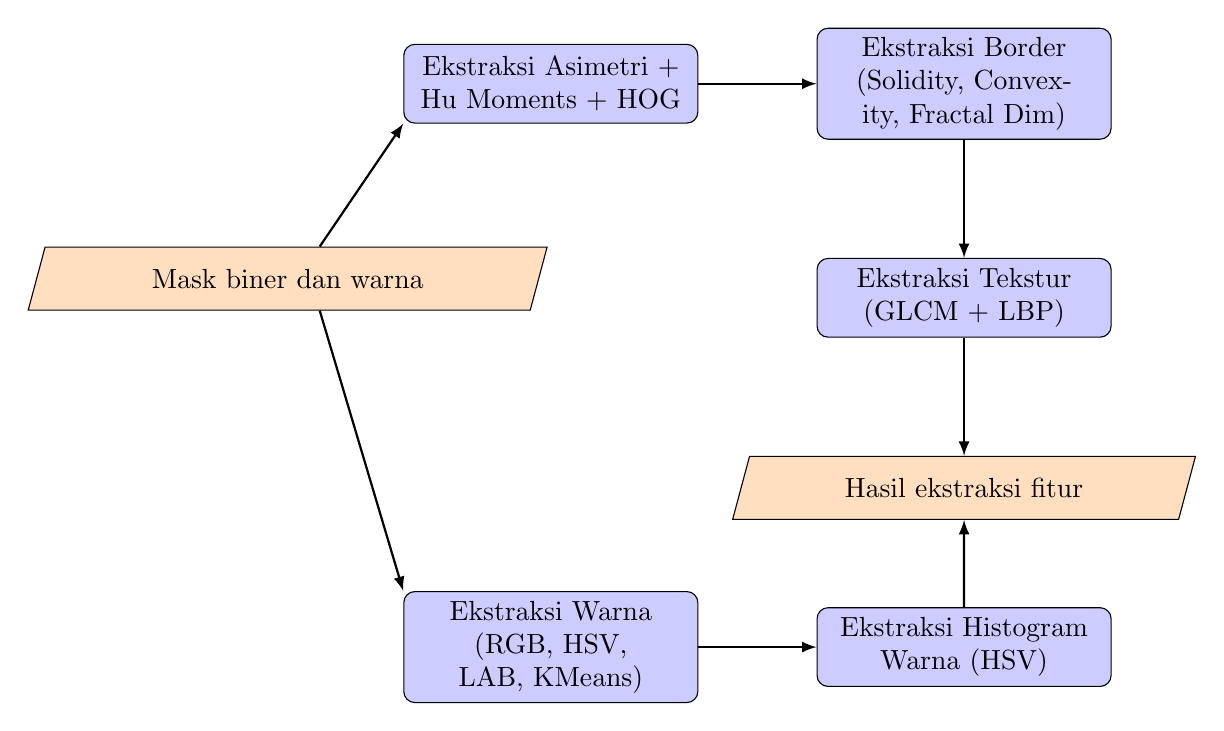
\begin{tikzpicture}[
      node distance=15mm,
      proc/.style={
          rectangle,
          draw,
          rounded corners,
          align=center,
          minimum width=30mm,
          minimum height=10mm,
          text width=35mm,
          fill=blue!20
        },
      io/.style={
          trapezium,
          trapezium left angle=75,
          trapezium right angle=105,
          draw,
          align=center,
          minimum width=25mm,
          minimum height=8mm,
          fill=orange!25
        },
      term-start/.style={
          circle,
          draw,
          align=center,
          minimum size=10mm,
          fill=green!25
        },
      term-finish/.style={
          circle,
          draw,
          align=center,
          minimum size=10mm,
          fill=red!25
        },
      arrow/.style={
          -latex,
          thick
        }
    ]

    % Start
    \node[io] (mask) {Mask biner dan warna};

    % Branch 1: Mask Biner
    \node[proc, above right=of mask, yshift=5mm] (biner_asym) {Ekstraksi Asimetri + Hu Moments + HOG};
    \node[proc, right=of biner_asym] (biner_border) {Ekstraksi Border (Solidity, Convexity, Fractal Dim)};
    \node[proc, below=of biner_border] (biner_texture) {Ekstraksi Tekstur (GLCM + LBP)};

    % Branch 2: Mask Berwarna
    \node[proc, below right=of mask, yshift=-25mm] (color_feats) {Ekstraksi Warna (RGB, HSV, LAB, KMeans)};
    \node[proc, right=of color_feats] (hist) {Ekstraksi Histogram Warna (HSV)};

    % Hasil
    \node[io, below=of biner_texture] (hasil) {Hasil ekstraksi fitur};

    % Arrows
    \draw[arrow] (mask.north east) -- (biner_asym.south west);
    \draw[arrow] (mask.south east) -- (color_feats.north west);

    % Biner branch
    \draw[arrow] (biner_asym) -- (biner_border);
    \draw[arrow] (biner_border) -- (biner_texture);

    % Color branch
    \draw[arrow] (color_feats) -- (hist);

    % Hasil
    \draw[arrow] (biner_texture) -- (hasil.north);
    \draw[arrow] (hist) -- (hasil.south);
  \end{tikzpicture}

  \caption{Pembagian Ekstraksi fitur citra dermoskopik berdasarkan mask yang digunakan}
  \label{fig:feature_extraction}
\end{figure}

\paragraph{1. Asimetri (Asymmetry)}
Citra lesi dipotong berdasarkan bounding box mask dan diubah ukurannya menjadi $128 \times 128$ piksel. Kemudian dilakukan perbandingan dengan versi citra yang dibalik horizontal dan vertikal, lalu dihitung selisih absolut rata-rata untuk menilai tingkat asimetri. Selain itu, \textit{Hu Moments} dan HOG (\textit{Histogram of Oriented Gradients}) juga dihitung untuk merepresentasikan bentuk dan tekstur lokal lesi.

\paragraph{2. Border (Batas Lesi)}
Menggunakan kontur dari mask, dihitung \textit{convex hull}, luas dan keliling asli serta keliling hull. Dari sini dihitung fitur \textit{solidity} dan \textit{convexity}. Fractal dimension juga dihitung dari kontur tepi untuk menangkap kompleksitas bentuk lesi.

\paragraph{3. Warna (Color)}
Fitur warna diekstraksi dari piksel di dalam mask dalam ruang warna RGB, HSV, dan LAB. Statistik dasar seperti standar deviasi tiap channel dihitung. Selain itu, K-Means clustering dengan 3 cluster digunakan untuk mengukur sebaran warna (color spread) sebagai representasi heterogenitas warna lesi.

\paragraph{4. Diameter dan Area}
Luas, keliling, dan diameter maksimum lesi dihitung dari kontur untuk mendukung karakteristik ukuran dan bentuk.

\paragraph{5. Tekstur (GLCM + LBP)}
Citra dikonversi ke grayscale.
\begin{itemize}
  \item \textbf{GLCM (Gray Level Co-occurrence Matrix)}: Fitur kontras, dissimilarity, homogeneity, energy, korelasi, dan ASM dihitung dari area mask untuk menangkap pola tekstur lokal.
  \item \textbf{LBP (Local Binary Pattern)}: Histogram LBP dihitung dengan metode ``uniform'' untuk invarian terhadap rotasi, ditambah fitur statistik seperti energi dan entropi dari distribusi LBP.
\end{itemize}

\paragraph{6. Histogram Warna}
Histogram warna HSV dihitung dengan 8 bins per channel untuk menangkap distribusi warna pada lesi. Nilai histogram dinormalisasi agar independen terhadap ukuran lesi.

\paragraph{Implementasi dan Penyimpanan}
Semua fitur digabungkan dalam satu \textit{DataFrame} dan disimpan ke file CSV (\texttt{features\_ABCD\_final.csv}) untuk tahap selanjutnya. Fitur-fitur ini siap digunakan untuk klasifikasi melanoma, baik menggunakan model \textit{machine learning} tradisional maupun metode \textit{deep learning} berbasis tabular input.

\subsection{Seleksi Fitur}
Seleksi fitur bertujuan untuk memilih subset fitur yang paling relevan dengan target klasifikasi, sekaligus mengurangi dimensi dataset agar model lebih efisien dan mengurangi risiko \textit{overfitting}. Pada penelitian ini, digunakan dua pendekatan seleksi fitur: \textbf{Principal Component Analysis (PCA)} dan \textbf{Chi-Square}.

\subsubsection{Principal Component Analysis (PCA)}
PCA adalah metode reduksi dimensi yang mentransformasikan fitur asli ke dalam himpunan baru \textit{principal components} yang saling ortogonal. Komponen-komponen ini disusun berdasarkan varian data, sehingga komponen pertama menyimpan varian terbesar, komponen kedua menyimpan varian terbesar kedua, dan seterusnya.

Langkah-langkah PCA secara umum adalah:
\begin{enumerate}
  \item Standarisasi fitur agar memiliki rata-rata nol dan variansi satu.
  \item Hitung matriks kovarians dari fitur standar.
  \item Lakukan dekomposisi nilai eigen (\textit{eigen decomposition}) untuk mendapatkan nilai eigen dan vektor eigen.
  \item Pilih sejumlah komponen utama yang menangkap persentase varian tertentu (misal 95\%) sebagai fitur akhir.
\end{enumerate}

Keuntungan PCA:
\begin{itemize}
  \item Mengurangi redundansi antar fitur yang saling berkorelasi.
  \item Mempercepat proses pelatihan model karena jumlah fitur berkurang.
  \item Mempertahankan informasi penting meskipun dimensi dikurangi.
\end{itemize}

\subsubsection{Chi-Square}
Uji chi-square digunakan untuk mengukur hubungan antara setiap fitur dengan kelas target. Konsep dasarnya adalah membandingkan frekuensi pengamatan dengan frekuensi yang diharapkan jika tidak ada hubungan antara fitur dan kelas.

Langkah-langkah seleksi fitur dengan chi-square:
\begin{enumerate}
  \item Untuk setiap fitur, buat tabel kontingensi yang menunjukkan distribusi nilai fitur terhadap kelas target.
  \item Hitung nilai chi-square untuk masing-masing fitur menggunakan rumus:
        \[
          \chi^2 = \sum \frac{(O_i - E_i)^2}{E_i}
        \]
        di mana $O_i$ adalah frekuensi yang diamati dan $E_i$ adalah frekuensi yang diharapkan.
  \item Fitur dengan nilai chi-square tinggi dianggap memiliki hubungan signifikan dengan kelas target dan dipilih untuk model.
\end{enumerate}

Keuntungan chi-square:
\begin{itemize}
  \item Memungkinkan pemilihan fitur yang paling berpengaruh terhadap klasifikasi.
  \item Sederhana dan cepat untuk dataset dengan banyak fitur.
  \item Efektif untuk fitur diskrit atau numerik yang telah dikategorikan.
\end{itemize}
Dengan kombinasi ini, diharapkan fitur akhir yang digunakan memiliki informasi maksimal, bebas dari redundansi, dan siap digunakan untuk proses klasifikasi dengan efisiensi tinggi.

\subsection{Klasifikasi}
Setelah fitur diekstraksi dan dilakukan seleksi fitur, tahap selanjutnya adalah klasifikasi untuk membedakan citra lesi menjadi kelas \textit{benign} dan \textit{malignant}. Pada penelitian ini, digunakan dua metode klasifikasi: \textbf{Support Vector Machine (SVM)} dan \textbf{Random Forest}.

\subsubsection{Support Vector Machine (SVM)}
SVM adalah algoritma pembelajaran \textit{supervised} yang bertujuan menemukan \textit{hyperplane} optimal yang memisahkan kelas-kelas pada ruang fitur. Hyperplane ini memaksimalkan margin antara kelas, sehingga model lebih tahan terhadap kesalahan klasifikasi pada data baru.

Beberapa detail implementasi SVM pada penelitian ini:
\begin{itemize}
  \item \textbf{Kernel}: RBF (\textit{Radial Basis Function}) digunakan untuk menangani data yang tidak linier.
  \item \textbf{Parameter C}: Mengatur toleransi kesalahan pada data pelatihan.
  \item \textbf{Parameter Gamma}: Mengatur pengaruh satu data terhadap bentuk hyperplane.
\end{itemize}

Keunggulan SVM:
\begin{itemize}
  \item Efektif untuk dataset dengan dimensi tinggi.
  \item Memiliki mekanisme margin yang meminimalkan risiko \textit{overfitting}.
  \item Cocok untuk dataset medis yang biasanya memiliki jumlah sampel terbatas.
\end{itemize}

\subsubsection{Random Forest}
Random Forest adalah metode \textit{ensemble learning} berbasis pohon keputusan, yang membangun banyak pohon secara acak dan mengambil keputusan mayoritas (\textit{majority voting}) untuk klasifikasi.

Detail implementasi Random Forest pada penelitian ini:
\begin{itemize}
  \item \textbf{Jumlah pohon}: Misal 100 pohon untuk mencapai kestabilan prediksi.
  \item \textbf{Fitur per split}: Setiap pohon hanya menggunakan subset fitur acak untuk memecah node.
  \item \textbf{Mekanisme voting}: Kelas akhir ditentukan berdasarkan mayoritas hasil dari semua pohon.
\end{itemize}

Keunggulan Random Forest:
\begin{itemize}
  \item Tahan terhadap \textit{overfitting} karena \textit{bagging} dan penggunaan banyak pohon.
  \item Mampu menangani fitur numerik dan kategorikal.
  \item Memberikan informasi penting tentang kontribusi masing-masing fitur (\textit{feature importance}).
\end{itemize}

\subsubsection{Evaluasi Kinerja Klasifikasi}
Kedua model dievaluasi menggunakan metrik:
\begin{itemize}
  \item \textbf{Akurasi}: Persentase prediksi benar dari total prediksi.
  \item \textbf{Precision, Recall, F1-Score}: Mengukur performa model terhadap kelas \textit{malignant} dan \textit{benign}.
\end{itemize}

\section{Hasil dan Pembahasan}
Pada tahap ini dijelaskan hasil dari eksperimen yang dilakukan.






\subsection{Dataset yang digunakan}
Sebagaimana yang disebutkan pada Bagian~\ref{section:dataset}, Dataset yang digunakan adalah Dataset ISIC 2016 Task 3 yang memang ditujukan untuk klasifikasi melanoma.

Setelah dilakukan ekstraksi fitur, didapatkan dataset tabular dalam format file CSV (\texttt{features\_ABCD\_final.csv}) yang terdiri dari 900 baris dan 67 kolom sebagaimana yang ditunjukkan pada Tabel~\ref{tab:fitur_ekstraksi}.

\begin{table}[H]
  \centering
  \begin{tabular}{|p{3cm}|p{12cm}|} % kolom pertama 3cm, kedua 12cm
    \hline
    \textbf{Kategori Fitur} & \textbf{Nama Kolom}                                                                                                                                                                            \\
    \hline
    Identitas               & image\_id, label                                                                                                                                                                               \\
    Asimetri                & asym\_total, hu\_0, hu\_1, hu\_2, hu\_3, hu\_4, hu\_5, hu\_6, hog\_mean, hog\_var                                                                                                              \\
    Batas / Border          & solidity, convexity, fractal\_dim                                                                                                                                                              \\
    Warna                   & std\_R, std\_G, std\_B, std\_H, std\_S, std\_V, color\_spread                                                                                                                                  \\
    Ukuran / Diameter       & area, perimeter, max\_diameter                                                                                                                                                                 \\
    Tekstur (GLCM)          & glcm\_contrast, glcm\_dissimilarity, glcm\_homogeneity, glcm\_energy, glcm\_correlation, glcm\_ASM                                                                                             \\
    Tekstur (LBP)           & lbp\_bin\_0, lbp\_bin\_1, lbp\_bin\_2, lbp\_bin\_3, lbp\_bin\_4, lbp\_bin\_5, lbp\_bin\_6, lbp\_bin\_7, lbp\_bin\_8, lbp\_bin\_9, lbp\_energy, lbp\_entropy                                    \\
    Histogram Warna (HSV)   & hist\_H\_bin\_0, hist\_H\_bin\_1, hist\_H\_bin\_2, hist\_H\_bin\_3, hist\_H\_bin\_4, hist\_H\_bin\_5, hist\_H\_bin\_6, hist\_H\_bin\_7, hist\_S\_bin\_0, hist\_S\_bin\_1, ..., hist\_V\_bin\_7 \\
    \hline
  \end{tabular}
  \caption{Ringkasan fitur ekstraksi dari dataset ISIC 2016.}
  \label{tab:fitur_ekstraksi}
\end{table}




\subsection{Lingkungan pengujian}
Pengujian manual dilakukan menggunakan Jupyter Notebook dengan bahasa pemrograman Python 3.12.2 dengan spesifikasi \textit{device} laptop HP Pavilion Gaming 5 adalah CPU AMD Ryzen 5 5600H, GPU RTX 3050 dan RAM 16 GB yang dijalankan di Windows 11 64 bit.

\subsection{Hasil}
\subsubsection{Statistik Dataset}\label{section:statistik-dataset}
Setelah mengimpor data csv, dilakukan beberapa eksplorasi visual statistik dataset.

\begin{figure}[H]
  \centering
  \includegraphics[width=1\linewidth]{images/distribusi-kelas.pdf}
  \caption{Distribusi tiap kelas}
  \label{fig:distribusi-kelas}
\end{figure}

Gambar~\ref{fig:distribusi-kelas} menampilkan distribusi tiap kelas dengan kelas \textit{benign} memiliki 727 instans, sementara kelas \textit{malignant} memiliki 173 instans. Kondisi ini merupakan kondisi \textit{data imbalance} yang perlu ditangani lebih lanjut.

\subsubsection{Hasil Ekstraksi Fitur}
Setelah itu, dilakukan beberapa visualisasi untuk melihat hasil dari ekstraksi fitur.

\begin{figure}[H]
  \centering
  \includegraphics[width=1\linewidth]{images/correlation-matrix.pdf}
  \caption{Matriks korelasi tiap kolom}
  \label{fig:correlation-matrix}
\end{figure}

Gambar~\ref{fig:correlation-matrix} menampilkan matriks korelasi tiap data numerik. Dapat dilihat bahwa kolom-kolom dengan kategori yang sama, sebagaimana pada Tabel~\ref{tab:fitur_ekstraksi}, memiliki korelasi yang cukup tinggi yang ditunjukkan oleh terbentuknya kotak persegi di sepanjang diagonal.

\begin{figure}[H]
  \centering
  \includegraphics[width=1\linewidth]{images/distribusi-fitur.pdf}
  \caption{Boxplot beberapa fitur penting}
  \label{fig:boxplot}
\end{figure}

Gambar~\ref{fig:boxplot} menampilkan boxplot beberapa fitur penting, seperti \textit{asym\_otal, hog\_mean, std\_S}, dan \textit{max\_diameter}. Dapat dilihat bahwa keempatnya merupakan fitur-fitur yang lemah karena distribusinya mirip setelah distandarisasi.

\begin{figure}[H]
  \centering
  \includegraphics[width=1\linewidth]{images/visualisasi-tsne.pdf}
  \caption{Distribusi tiap fitur berdasarkan kelas}
  \label{fig:tsne}
\end{figure}

Gambar~\ref{fig:tsne} menampilkan proyeksi data berdimensi tinggi ke dalam 2 dimensi untuk melihat keterpisahan data antara kelas kanker (\textit{malignant-oranye}) dan jinak (\textit{benign-biru}). Dari hasil visualisasi dapat dilihat bahwa terjadi tumpang tindih yang signifikan (\textit{significant overlap}) yang mana titik oranye tidak berkumpul dalam satu klaster yang terpisah. Titik-titik ini tersebar dan tercampur baur dengan titik biru. Hal ini juga mengisyaratkan bahwa tidak ada garis pemisah yang jelas (linear separability) yang memisahkan kedua kelas ini.

Selain itu, secara visual, titik biru jauh lebih banyak daripada titik oranye. Hal ini mengonfirmasi adanya \textit{data imbalance}, sebagaimana yang telah disebutkan di Bagian~\ref{section:statistik-dataset}.

Berdasarkan hal-hal di atas, sangat penting untuk melakukan seleksi fitur.


\subsubsection{Seleksi Fitur dan Hasil Klasifikasi}

Pada penelitian ini dilakukan dua pendekatan seleksi fitur, yaitu metode berbasis statistik (Chi-square) dan reduksi dimensi linier (Principal Component Analysis/PCA). Kedua hasil seleksi fitur tersebut kemudian diuji menggunakan model klasifikasi Support Vector Machine (SVM). Bagian ini menyajikan fitur-fitur terpilih, jumlah komponen PCA, serta analisis performa klasifikasi untuk masing-masing skenario.

\paragraph{Skenario 1: Chi-square + SVM (Fitur Asli Terbaik)}

Pada skenario pertama, seleksi fitur dilakukan menggunakan metode Chi-square ($ \chi^2 $) yang memilih fitur berdasarkan dependensi stokastik tertinggi terhadap label kelas. Dari 65 fitur awal, terpilih 10 fitur dengan nilai Chi-square tertinggi:

\begin{itemize}
  \item \textbf{Geometri:} \texttt{area}
  \item \textbf{Tekstur:} \texttt{glcm\_ASM}
  \item \textbf{Statistik Warna:} \texttt{std\_H}, \texttt{std\_V}
  \item \textbf{Histogram Warna:} \texttt{hist\_H\_bin\_3, 4, 5}, \texttt{hist\_S\_bin\_0}, \texttt{hist\_V\_bin\_1, 2}
\end{itemize}

\textbf{Analisis Fitur Terpilih:}
Dominasi fitur berbasis warna (Histogram Hue dan Saturation) serta standar deviasi (\texttt{std\_H}, \texttt{std\_V}) mengindikasikan bahwa variasi warna (variegation) merupakan diskriminator terkuat dalam dataset ini. Hal ini sejalan dengan kaidah klinis ABCD, di mana \textit{Color variegation} adalah indikator utama keganasan. Fitur \texttt{glcm\_ASM} (keseragaman tekstur) dan \texttt{area} juga terpilih, menandakan bahwa lesi ganas cenderung memiliki tekstur yang kurang seragam dan ukuran yang berbeda signifikan dari lesi jinak.

Model SVM dengan 10 fitur ini menghasilkan akurasi \textbf{0.7778}.

\begin{verbatim}
              precision    recall  f1-score   support

      benign       0.87      0.86      0.86       145
   malignant       0.43      0.46      0.44        35

    accuracy                           0.78       180
   macro avg       0.65      0.66      0.65       180
weighted avg       0.78      0.78      0.78       180
\end{verbatim}

Meskipun akurasi keseluruhan cukup baik, nilai \textit{recall} untuk kelas \textit{malignant} masih rendah (0.46). Artinya, model gagal mendeteksi lebih dari separuh kasus kanker (False Negative tinggi).

\paragraph{Skenario 2: PCA + SVM (Reduksi Dimensi)}

Skenario kedua menggunakan PCA untuk mentransformasi fitur ke dalam ruang dimensi baru yang ortogonal. Untuk mempertahankan 95\% variasi informasi (cumulative explained variance), PCA menghasilkan \textbf{29 komponen utama} (Principal Components).

Hasil klasifikasi menunjukkan penurunan performa dengan akurasi \textbf{0.7056}.

\begin{verbatim}
              precision    recall  f1-score   support

      benign       0.85      0.77      0.81       145
   malignant       0.32      0.46      0.38        35

    accuracy                           0.71       180
   macro avg       0.59      0.61      0.59       180
weighted avg       0.75      0.71      0.72       180
\end{verbatim}

\textbf{Analisis Penurunan Performa:}
Penggunaan 29 komponen PCA justru menghasilkan performa yang lebih rendah dibandingkan hanya menggunakan 10 fitur asli (Chi-square). Hal ini mengindikasikan dua hal:
\begin{enumerate}
  \item \textbf{Kehilangan Interpretasi Fisik:} PCA menggabungkan seluruh fitur secara linier. Fitur diskriminatif kuat (seperti \texttt{std\_H}) mungkin "terlarut" (diluted) ketika digabung dengan fitur-fitur lemah lainnya dalam komponen utama.
  \item \textbf{Curse of Dimensionality:} Jumlah input 29 komponen relatif besar dibandingkan jumlah sampel latih yang terbatas, yang berpotensi menyulitkan SVM dalam menemukan \textit{hyperplane} optimal (overfitting terhadap noise).
\end{enumerate}

\paragraph{Diskusi Perbandingan dan Isu Ketimpangan Kelas}

Perbandingan ringkas performa kedua skenario disajikan pada Tabel \ref{tab:perbandingan}.

\begin{table}[h]
  \centering
  \caption{Perbandingan Metrik Evaluasi Chi-square vs PCA pada Kelas Malignant}
  \label{tab:perbandingan}
  \begin{tabular}{|l|c|c|c|}
    \hline
    \textbf{Metode Seleksi} & \textbf{Precision (Mal)} & \textbf{Recall (Mal)} & \textbf{F1-Score (Mal)} \\ \hline
    Chi-square (10 Fitur)   & \textbf{0.43}            & 0.46                  & \textbf{0.44}           \\ \hline
    PCA (29 Komponen)       & 0.32                     & 0.46                  & 0.38                    \\ \hline
  \end{tabular}
\end{table}

Berdasarkan Tabel~\ref{tab:perbandingan}, secara umum, \textbf{Chi-square terbukti lebih efektif} dibanding PCA dalam kasus ini. Penggunaan subset fitur asli yang spesifik lebih mampu menangkap karakteristik lesi dibanding transformasi global PCA.

Namun, kendala utama yang terlihat pada kedua skenario adalah rendahnya nilai \textit{Recall} dan \textit{Precision} pada kelas \textit{malignant}. Hal ini sangat dipengaruhi oleh \textbf{ketimpangan data (imbalanced dataset)} di mana jumlah sampel \textit{benign} (145) jauh mendominasi \textit{malignant} (35). Model cenderung bias ke kelas mayoritas, sehingga menghasilkan banyak False Negative pada kelas kanker. Untuk pengembangan selanjutnya, teknik penanganan data tidak seimbang seperti SMOTE (\textit{Synthetic Minority Over-sampling Technique}) atau \textit{class weighting} sangat disarankan untuk meningkatkan sensitivitas deteksi kanker.

Gambar~\ref{fig:confusion-matrix-seleksi} menampilkan hasil \textit{confusion matrix} kedua seleksi fitur.
\begin{figure}[H]
  \centering
  \includegraphics[width=1\linewidth]{images/confusion-matrix-seleksi.pdf}
  \caption{Hasil \textit{confusion matrix} kedua seleksi fitur.}
  \label{fig:confusion-matrix-seleksi}
\end{figure}


\subsubsection{Hasil Eksperimen Lanjutan}
Selain skenario utama menggunakan Chi-square dan PCA, dilakukan pula beberapa eksperimen tambahan, termasuk penerapan SMOTE serta penggunaan model lain seperti Random Forest. Bagian berikut merangkum seluruh hasil tersebut.

\paragraph{Skenario 1: Chi-Square + SVM (Dengan SMOTE)}
Metode Chi-square dipilih untuk mengambil 10 fitur terbaik, yaitu:
\textit{std\_H, std\_V, area, glcm\_ASM, hist\_H\_bin\_3, hist\_H\_bin\_4, hist\_H\_bin\_5, hist\_S\_bin\_0, hist\_V\_bin\_1, hist\_V\_bin\_2}.

\begin{verbatim}
              precision    recall  f1-score   support
benign            0.85      0.82      0.84       145
malignant         0.35      0.40      0.37        35
accuracy                              0.74       180
macro avg         0.60      0.61      0.60       180
weighted avg      0.75      0.74      0.75       180
\end{verbatim}

\paragraph{Skenario 2: PCA + SVM (Dengan SMOTE)}
Jumlah fitur awal adalah 65, dan PCA mempertahankan 29 komponen dengan varian terjelaskan sebesar 95.45\%.

\begin{verbatim}
              precision    recall  f1-score   support
benign            0.83      0.81      0.82       145
malignant         0.28      0.31      0.30        35
accuracy                              0.71       180
macro avg         0.56      0.56      0.56       180
weighted avg      0.72      0.71      0.72       180
\end{verbatim}

\paragraph{Skenario 3: SVM Full Features (Baseline)}
Pada baseline ini seluruh 65 fitur digunakan tanpa reduksi dimensi.

\begin{verbatim}
              precision    recall  f1-score   support
benign            0.83      0.81      0.82       145
malignant         0.27      0.29      0.28        35
accuracy                              0.71       180
macro avg         0.55      0.55      0.55       180
weighted avg      0.72      0.71      0.71       180
\end{verbatim}

\paragraph{Skenario 3b: SVM Full Features + SMOTE}
SMOTE diterapkan pada data training, namun performa tidak berubah signifikan.

\begin{verbatim}
              precision    recall  f1-score   support
benign            0.83      0.81      0.82       145
malignant         0.27      0.29      0.28        35
accuracy                              0.71       180
macro avg         0.55      0.55      0.55       180
weighted avg      0.72      0.71      0.71       180
\end{verbatim}

\paragraph{Skenario 4: Chi-Square + Random Forest (Dengan SMOTE)}
Model Random Forest dilatih pada 10 fitur terbaik Chi-square.

\begin{verbatim}
accuracy: 0.7611

              precision    recall  f1-score   support
benign            0.83      0.88      0.86       145
malignant         0.35      0.26      0.30        35
accuracy                              0.76       180
macro avg         0.59      0.57      0.58       180
weighted avg      0.74      0.76      0.75       180
\end{verbatim}

\paragraph{Skenario 5: PCA + Random Forest (Dengan SMOTE)}
Model Random Forest dilatih menggunakan 29 komponen PCA.

\begin{verbatim}
accuracy: 0.7444

              precision    recall  f1-score   support
benign            0.82      0.87      0.85       145
malignant         0.30      0.23      0.26        35
accuracy                              0.74       180
macro avg         0.56      0.55      0.55       180
weighted avg      0.72      0.74      0.73       180
\end{verbatim}

\paragraph{Skenario 6: Full Features + Random Forest (Dengan SMOTE)}
Pada skenario ini digunakan seluruh 65 fitur.

\begin{verbatim}
accuracy: 0.7889

              precision    recall  f1-score   support
benign            0.84      0.91      0.87       145
malignant         0.43      0.29      0.34        35
macro avg         0.64      0.60      0.61       180
weighted avg      0.76      0.79      0.77       180
\end{verbatim}

5 fitur paling penting:
\textit{solidity (0.0289), hist\_V\_bin\_0 (0.0277), hog\_var (0.0268), hist\_H\_bin\_4 (0.0267), hist\_V\_bin\_2 (0.0266)}.

\begin{table*}[h!]
  \centering
  \caption{Perbandingan hasil seluruh skenario eksperimen yang dilakukan.}
  \label{tab:perbandingan_skenario}
  \renewcommand{\arraystretch}{1.2}
  \begin{tabular}{|p{3.5cm}|c|c|c|c|}
    \hline
    \textbf{Skenario}                     & \textbf{Accuracy} & \textbf{Precision (Mal)} & \textbf{Recall (Mal)} & \textbf{F1-score (Mal)} \\
    \hline

    Chi-Square + SVM + SMOTE              &
    0.74                                  &
    0.35                                  &
    0.40                                  &
    0.37                                                                                                                                   \\
    \hline

    PCA + SVM + SMOTE                     &
    0.71                                  &
    0.28                                  &
    0.31                                  &
    0.30                                                                                                                                   \\
    \hline

    SVM Full Features (Baseline)          &
    0.71                                  &
    0.27                                  &
    0.29                                  &
    0.28                                                                                                                                   \\
    \hline

    SVM Full Features + SMOTE             &
    0.71                                  &
    0.27                                  &
    0.29                                  &
    0.28                                                                                                                                   \\
    \hline

    Chi-Square + Random Forest + SMOTE    &
    0.76                                  &
    0.35                                  &
    0.26                                  &
    0.30                                                                                                                                   \\
    \hline

    PCA + Random Forest + SMOTE           &
    0.74                                  &
    0.30                                  &
    0.23                                  &
    0.26                                                                                                                                   \\
    \hline

    Full Features + Random Forest + SMOTE &
    0.79                                  &
    0.43                                  &
    0.29                                  &
    0.34                                                                                                                                   \\
    \hline
  \end{tabular}
\end{table*}


Berdasarkan Tabel~\ref{tab:perbandingan_skenario}, dari seluruh eksperimen, performa terbaik diperoleh menggunakan \textbf{Random Forest dengan seluruh fitur} dengan akurasi 78.89\%. Untuk model SVM, \textbf{Chi-square memberikan performa terbaik} dengan akurasi 77.78\%, melampaui PCA dan baseline.

\subsection{Diskusi}

Bagian ini membahas implikasi hasil eksperimen, faktor penyebab performa model, serta keterbatasan pendekatan yang digunakan. Secara umum, hasil menunjukkan bahwa pemilihan fitur memiliki dampak yang jauh lebih besar terhadap performa klasifikasi dibandingkan reduksi dimensi linier seperti PCA. Selain itu, ketidakseimbangan kelas (\textit{class imbalance}) terbukti menjadi faktor paling dominan yang memengaruhi rendahnya performa deteksi melanoma.

\subsubsection{Pengaruh Seleksi Fitur}
Sebagaimana Tabel~\ref{tab:perbandingan}, pendekatan Chi-square konsisten menghasilkan performa yang lebih baik dibanding PCA pada model SVM. Hal ini menunjukkan bahwa mempertahankan fitur-fitur dengan hubungan statistik paling kuat terhadap label lebih efektif dibanding mentransformasikan seluruh fitur ke ruang baru. Fitur-fitur berbasis warna (seperti \texttt{std\_H}, \texttt{std\_V}, dan histogram HSV) mendominasi daftar fitur terpilih, yang mengindikasikan bahwa variasi warna merupakan indikator klinis yang kuat sebagaimana konsep \textit{Color variegation} pada kaidah ABCD.

Berbeda dengan itu, PCA cenderung melarutkan kontribusi fitur-fitur penting ketika menggabungkannya secara linier. Meskipun PCA mempertahankan 95\% variasi data, komponen utama tidak menjamin mempertahankan informasi diskriminatif yang relevan untuk klasifikasi. Ini menyebabkan performa model turun meskipun jumlah fitur yang digunakan lebih banyak.

\subsubsection{Performa Model dan Perbandingan SVM vs Random Forest}
Berdasarkan Tabel~\ref{tab:perbandingan_skenario}, model SVM menunjukkan kinerja terbaik ketika digabungkan dengan fitur hasil seleksi Chi-square. Namun, ketika seluruh fitur digunakan, Random Forest justru memberikan performa tertinggi (78.89\%). Hal ini dapat dijelaskan oleh sifat dasar Random Forest yang mampu menangkap hubungan nonlinier antar fitur serta tidak sensitif terhadap fitur yang saling berkorelasi.

Selain itu, analisis \textit{feature importance} pada Random Forest memperlihatkan bahwa fitur-fitur geometris (\textit{solidity}) dan tekstur (\textit{hog\_var}) ternyata termasuk yang paling berkontribusi. Temuan ini menarik karena memperlihatkan bahwa informasi bentuk dan tekstur tetap penting, meskipun warna mendominasi pada SVM dengan seleksi Chi-square.

\subsubsection{Dampak Ketidakseimbangan Kelas}
Isu paling kritis pada seluruh eksperimen adalah rendahnya \textit{recall} kelas \textit{malignant}. Hal ini menunjukkan bahwa sebagian besar kasus melanoma gagal terdeteksi. Ketidakseimbangan jumlah sampel (\(145\) benign vs \(35\) malignant) membuat model cenderung bias ke kelas mayoritas. Upaya penanganan melalui SMOTE meningkatkan keseimbangan data latih, tetapi belum memberikan perbaikan signifikan pada performa, terutama untuk SVM.

Fenomena ini umum terjadi pada data medis, di mana jumlah sampel kasus penyakit biasanya jauh lebih sedikit dibandingkan sampel normal. Dengan demikian, pendekatan lain seperti \textit{class weighting}, \textit{focal loss}, atau metode augmentasi spesifik citra lesi mungkin diperlukan untuk memperoleh performa yang lebih baik.

\subsubsection{Keterbatasan dan Peluang Pengembangan}
Hasil yang diperoleh memperlihatkan bahwa meskipun fitur-fitur hand-crafted dari kaidah ABCD relatif informatif, performanya belum mampu mencapai sensitivitas yang layak untuk deteksi klinis. Beberapa keterbatasan utama penelitian ini antara lain:

\begin{enumerate}
  \item Ketergantungan pada fitur manual (hand-crafted) yang terbatas pada representasi tertentu.
  \item Jumlah data yang sedikit sehingga model sulit belajar pola kompleks.
  \item Variasi citra ISIC (pencahayaan, resolusi, artefak kulit) yang tidak sepenuhnya ditangani.
\end{enumerate}

Penelitian lanjutan dapat mengintegrasikan fitur deep learning (misalnya melalui transfer learning CNN) dengan fitur ABCD untuk menghasilkan representasi hibrid yang lebih kuat. Selain itu, metode cost-sensitive learning sangat relevan untuk mengurangi bias terhadap kelas mayoritas.

Secara keseluruhan, hasil studi menunjukkan pentingnya strategi seleksi fitur, teknik penanganan data tidak seimbang, serta pemilihan model yang mampu menangkap interaksi nonlinier untuk meningkatkan kinerja deteksi melanoma berbasis citra.


% \begin{figure}[H]
%     \centering
%     \includegraphics[width=1\linewidth]{images/diagram alir.pdf}
%     \caption{Diagram alir metode yang diusulkan.}
%     \label{fig:diagramalir}
% \end{figure}


% \begin{table}[H]
%     \centering
%     \begin{tabular}{c|c|c}
%         No. & Kelas & Jumlah data \\
%         1 & Maju & 22 \\
%         2 & Mundur & 26 \\
%         3 & Berhenti & 23 \\
%         4 & Kiri & 25 \\
%         5 & Kanan & 26 \\
%     \end{tabular}
%     \caption{Banyaknya data tiap kelas.}
%     \label{tab:rincianjumlahdata}
% \end{table}


\section{Kesimpulan}

Berdasarkan hasil dan analisis yang telah dilakukan, dapat disimpulkan bahwa:

Kode tersedia pada \textit{repository} GitHub \url{https://github.com/khalilullahalfaath/RFPP---Melanoma-Classification-Handcrafted-Features-}.

\newpage

% Daftar pustaka
\printbibliography

\end{document}
